\documentclass[border=10pt]{standalone}

\usepackage{tikz}
\usepackage{tikzsymbols}
\usetikzlibrary{calc,patterns,shapes.geometric}

\def\centerarc[#1](#2)(#3:#4:#5){\draw[#1] ($(#2)+({#5*cos(#3)},{#5*sin(#3)})$) arc (#3:#4:#5);}

\begin{document}
	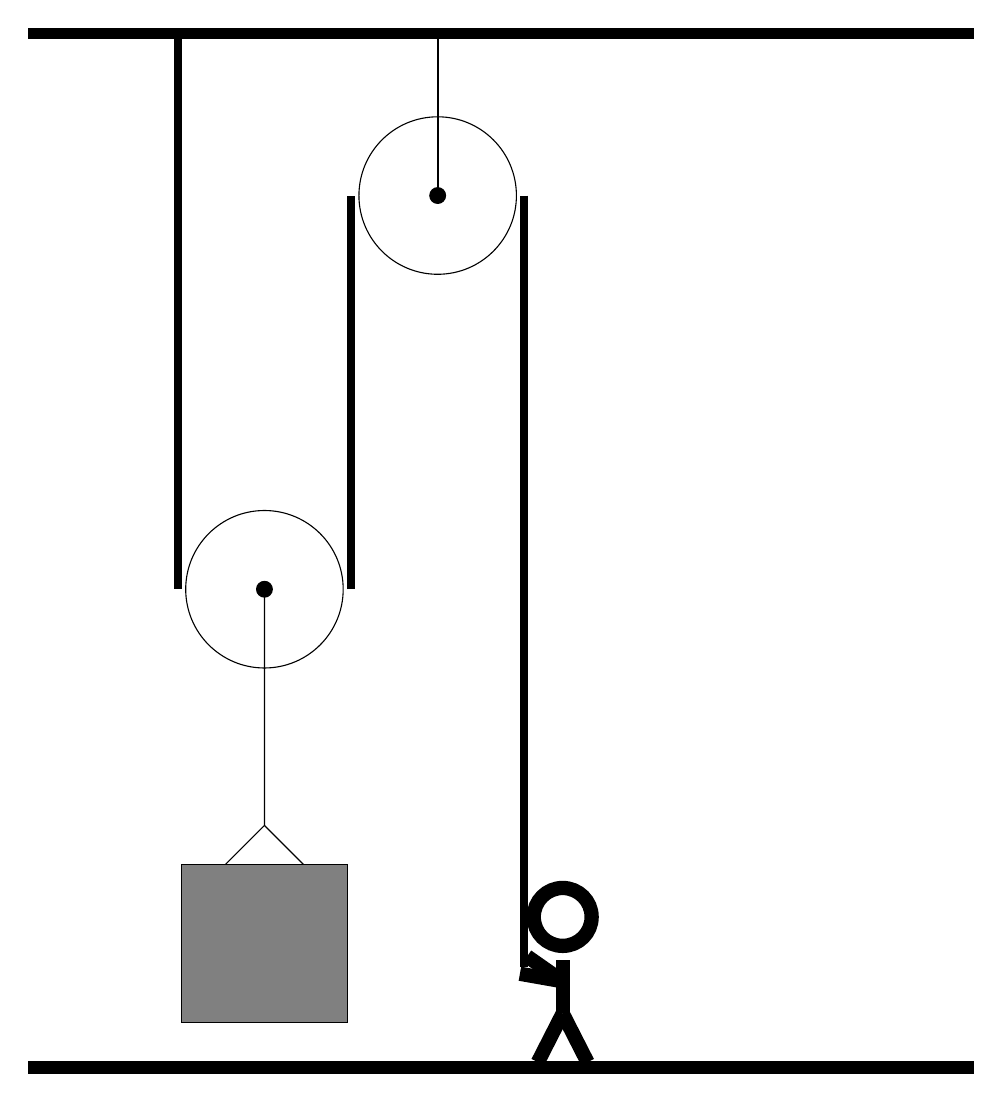
\begin{tikzpicture}
		%%%%% START %%%%%
		\draw[fill=black] (-2, 10) rectangle (10, 10.125);
		
		\draw (3.2, 8.0) circle (1);
		\draw[fill=black] (3.2, 8.0) circle (0.1);
		\draw[thick] (3.2, 8.0) -- (3.2, 10);
		
		\draw (1, 3.0) circle (1);
		\draw[fill=black] (1, 3.0) circle (0.1);
		
		\draw (1, 3.0) -- (1, 0) -- (0.5, -0.5);
		\draw (1, 0) -- (1.5, -0.5);
		\draw[fill=black!50] (-0.05, -0.5) rectangle (2.05, -2.5);
		
		\draw[line width=1mm] (-0.1, 10) -- (-0.1, 3.0);
		\centerarc[line width=1mm](1, 3.0)(180:360:1.1);
		\draw[line width=1mm](2.1, 3.0) -- (2.1, 8.0);
		\centerarc[line width=1mm](3.2, 8.0)(0:180:1.1);
		\draw[line width=1mm](4.3, 8.0) -- (4.3, -1.8);
		
		\node at (4.7, -1.9) {\Strichmaxerl[10][-35][170]};
		
		\draw[fill=black] (-2, -3) rectangle (10, -3.15);
		%%%%% END %%%%%
	\end{tikzpicture}
\end{document}